% partes/parte2/cap07.tex
\chapter{\textit{Customer journey}: del interés a la satisfacción y su mapeo}
\label{cap:07}

\begin{cajaFicha}
\begin{description}
  \item[Unidad temática] II — Proceso de toma de decisión de compra digital.
  \item[Temas del programa] 2.2 \textit{Customer journey} (recorrido del consumidor digital): 2.2.1 Atención; 2.2.2 Interés; 2.2.3 Deseo; 2.2.4 Acción; 2.2.5 Satisfacción; 2.2.6 Mapeo del \textit{customer journey}.
  \item[Horas] Teoría 2.0 · Práctica 5.0 · Aprendizaje autónomo 2.0 (asignación tentativa; ver Anexo B del prompt de proyecto, anomalía 4).
  \item[Competencia de la unidad] Examina el proceso de toma de decisiones de compra del consumidor digital a partir de su recorrido y figuras participantes.
  \item[Resultados de aprendizaje observables] Al concluir el capítulo, el estudiante:
  \begin{enumerate}
    \item recorre las cinco etapas del modelo AIDAS y las traduce a puntos de contacto, datos y métricas digitales;
    \item explica por qué el embudo lineal describe mal el comportamiento observado y distingue la evidencia independiente de los marcos de consultoría;
    \item construye un mapa de recorrido y declara sus límites;
    \item modela un recorrido como cadena de Markov, calcula la probabilidad y el tiempo de conversión y compara tres modelos de atribución.
  \end{enumerate}
  \item[Prerrequisitos] Cap. 1--6.
\end{description}
\end{cajaFicha}

\section{Caso de apertura}

El modelo más citado del marketing no tiene un inventor claro. Cualquier
manual lo atribuye a Elias St.\ Elmo Lewis, quien lo habría formulado en 1898:
atraer la atención, mantener el interés, crear el deseo, obtener la acción. La
atribución circula desde 1925, cuando Edward K.\ Strong la afirmó en un libro
de psicología de las ventas. Durante un siglo se repitió sin consultar los
documentos de la época.

\textcite{iwamoto2024origenaida} sí los consultó. Revisó fuentes
originales, entre ellas los textos de la Sheldon School, y encontró que no
hay evidencia primaria de que Lewis formulara el prototipo en 1898. Arthur
Frederick Sheldon y Frank H.\ Dukesmith lo teorizaron antes y con mejor
sustento documental. El acrónimo AIDA, según el mismo estudio, apareció en 1921
con C.\ P.\ Russell, en la revista \textit{Printers' Ink}.

El caso enseña dos cosas. La primera: un modelo puede ser útil y su genealogía,
dudosa. La segunda, más importante para este capítulo: una narrativa que
repite un siglo no es evidencia. Esa cautela vale igual para los marcos
modernos del recorrido del consumidor, varios de los cuales vienen de
consultoras o de plataformas publicitarias.

\section{Desarrollo teórico}

\subsection{De AIDA a AIDAS: las cinco etapas del recorrido}
\label{sec:cap07-aidas}

El recorrido (\textit{customer journey}) describe el camino que sigue una
persona desde que se entera de una oferta hasta que la usa y opina sobre
ella. El programa oficial lo organiza en cinco etapas que corresponden al
modelo AIDAS: atención, interés, deseo, acción y satisfacción. La última letra
es una extensión posterior que cierra el ciclo hacia la poscompra y es la
que conecta con la etapa 2.1.5 del capítulo anterior.

Conviene separar el modelo original de su lectura digital. AIDA nació para
describir la venta personal y la publicidad impresa. Su traducción a
marketing digital, que se resume en el cuadro~\ref{tab:cap07-aidas}, es una
\emph{reinterpretación aplicada} y no una cita de Sheldon, Lewis ni Strong.

\begin{table}[!htb]
\centering
\begin{tabular}{@{}p{2.1cm}p{3.6cm}p{3.5cm}p{3.3cm}@{}}
\toprule
Etapa & Punto de contacto típico & Dato que deja & Métrica habitual \\
\midrule
Atención & Anuncio, publicación, resultado de búsqueda & Impresión, tiempo de visualización & Alcance, frecuencia \\
Interés & Visita al sitio, lectura de reseñas & Clic, tiempo en página, desplazamiento & Tasa de clics, páginas por sesión \\
Deseo & Producto guardado, comparación, carrito & Evento de \enquote{agregar al carrito} & Tasa de carrito, abandono de carrito \\
Acción & \textit{Checkout} y pago & Transacción & Tasa de conversión \\
Satisfacción & Entrega, soporte, reseña & Calificación, devolución, recompra & Recompra, recomendación \\
\bottomrule
\end{tabular}
\caption{Lectura digital de las cinco etapas AIDAS. Es una reinterpretación
aplicada del modelo, no su formulación original. Fuente: elaboración propia.}
\label{tab:cap07-aidas}
\end{table}

\subsubsection{Atención}
\progtag{2.2.1}
Es la etapa en que la oferta entra al campo perceptivo de la persona. En
digital, la atención se mide por exposición, pero exposición no es atención:
un anuncio puede cargarse en pantalla sin que nadie lo vea. Por eso la
métrica de una impresión describe una oportunidad y no un hecho psicológico.

\subsubsection{Interés}
\progtag{2.2.2}
La persona busca saber más. Su comportamiento deja huellas claras: abre la
página, lee, vuelve. El interés es también la etapa en que se activa la
búsqueda de información del Cap.~6 y en que pesan las reseñas de terceros.

\subsubsection{Deseo}
\progtag{2.2.3}
El interés se vuelve preferencia. La persona compara, guarda, imagina el
uso. Es la etapa más difícil de observar, porque ocurre dentro de la persona;
los datos solo capturan su sombra (un producto guardado, un carrito sin
pagar). Aquí la economía conductual del capítulo anterior
opera con más fuerza: el temporizador y la insignia de escasez buscan
convertir deseo en acción.

\subsubsection{Acción}
\progtag{2.2.4}
La compra. Es la única etapa que casi siempre se registra con precisión, y
por eso se la sobrevalora: se atribuye todo a lo que ocurrió justo antes del
pago. La sección~\ref{sec:cap07-lab} muestra cuánto distorsiona esa
costumbre.

\subsubsection{Satisfacción}
\progtag{2.2.5}
La persona usa el producto y contrasta su experiencia con lo que esperaba. El
canal digital vuelve visible esta etapa y la reinyecta al recorrido de otros
como reseña, calificación o recomendación. La satisfacción se define frente a la expectativa previa, como lo formaliza,
por ejemplo, el índice de satisfacción del cliente estadounidense
\parencite{fornell1996}. Una experiencia satisfactoria
produce recompra y recomendación; una mala, devolución o queja pública.

\subsection{Un marco contemporáneo: las 5A de Kotler}

\textcite{kotler2021marketing50} proponen las 5A (\textit{aware, appeal, ask,
act, advocate}: conocer, atraer, preguntar, actuar, recomendar) como sucesor
de AIDA para el marketing conectado. Añade dos ideas útiles: la fase de
\enquote{preguntar}, en que la persona consulta a pares y a la marca, y la de
\enquote{recomendar}, en que la satisfacción se convierte en influencia. Debe
leerse con la misma cautela que los demás marcos de consultoría: es una
propuesta con valor pedagógico y sin validación empírica independiente.

\begin{cajaFrontera}
\textbf{El recorrido no lineal: del embudo al bucle.} El embudo de conversión
(AIDA aplicada como secuencia estricta) sigue siendo un punto de partida
pedagógico. Describe mal lo que la gente hace. Tres piezas permiten ver por
qué, y conviene distinguir qué respaldo tiene cada una
(cuadro~\ref{tab:cap07-marcos}, figura~\ref{fig:cap07-bucle}).

\textcite{court2009consumer} introdujeron el \textit{consumer decision journey}
con un estudio propio de unos 20\,000 consumidores en cinco industrias y tres
países. Su hallazgo central es que las personas no bajan por el embudo:
agregan y quitan marcas a mitad del camino y regresan. Es investigación de una
consultora, no un artículo arbitrado. Sin embargo, la revisión sistemática de
\textcite{santos2021consumer}, publicada en una revista arbitrada, sitúa ese
modelo en un linaje más amplio (experiencia de cliente, comportamiento
social, trazado de recorridos) y respalda la idea general de que el
recorrido no es lineal.

El \textit{messy middle} de \textcite{google2020messy} describe el tramo
entre el disparador y la compra como un ir y venir entre \emph{explorar}
(sumar opciones) y \emph{evaluar} (reducirlas), influido por sesgos
cognitivos. Se basa en 310\,000 escenarios simulados de compra y es
investigación propietaria de una empresa que vende publicidad justo en ese
tramo. Eso no invalida el hallazgo. Obliga a declarar el conflicto de interés.

La distinción que importa es esta: la crítica al embudo lineal \emph{sí} tiene
respaldo académico independiente. Los modelos de marca (el recorrido de
McKinsey, el tramo caótico de Google) son marcos útiles con estudio propio, no
experimentos neutrales. Y en 2026 los asistentes de compra basados en IA
(Cap.~4) pueden absorber parte de la exploración y la evaluación, lo que
reabre la misma pregunta de fondo: quién reduce las opciones antes de la
decisión final.
\end{cajaFrontera}

\begin{figure}[!htb]
  \centering
  \resizebox{0.95\textwidth}{!}{% figuras/tikz/cap07-embudo-vs-bucle.tex
% Embudo lineal (AIDA) frente a recorrido en bucle (consumer decision journey / messy middle).
\begin{tikzpicture}[
    et/.style={rectangle, rounded corners, draw=guindaIPN, thick, fill=guindaIPNClara,
               minimum width=1.9cm, minimum height=0.8cm, align=center, font=\scriptsize},
    flecha/.style={-{Stealth[length=2.2mm]}, thick, draw=doradoIPN},
    retro/.style={-{Stealth[length=2.2mm]}, thick, draw=terracotaIPN, dashed},
    tit/.style={font=\small\bfseries, align=center}
  ]
  % --- Izquierda: embudo lineal
  \node[tit] at (0,3.7) {Embudo lineal};
  \node[et, minimum width=4.6cm] (a1) at (0,2.8) {Atención};
  \node[et, minimum width=3.7cm] (a2) at (0,1.7) {Interés};
  \node[et, minimum width=2.8cm] (a3) at (0,0.6) {Deseo};
  \node[et, minimum width=1.9cm] (a4) at (0,-0.5) {Acción};
  \foreach \a/\b in {a1/a2,a2/a3,a3/a4} { \draw[flecha] (\a) -- (\b); }
  \node[font=\tiny, text=grisIPN, align=center] at (0,-1.4) {una sola dirección;\\ el consumidor solo \enquote{baja}};

  % --- Derecha: bucle
  \node[tit] at (7.2,3.7) {Recorrido en bucle};
  \node[et] (b0) at (7.2,2.8) {Disparador};
  \node[et] (b1) at (5.4,1.1) {Exploración\\ (suma opciones)};
  \node[et] (b2) at (9.0,1.1) {Evaluación\\ (reduce opciones)};
  \node[et] (b3) at (7.2,-0.5) {Compra};
  \node[et] (b4) at (10.6,-0.5) {Uso y\\ reseña};
  \draw[flecha] (b0) -- (b1);
  \draw[retro] (b1.east) to[bend left=25] (b2.west);
  \draw[retro] (b2.west) to[bend left=25] (b1.east);
  \draw[flecha] (b2) -- (b3);
  \draw[flecha] (b3) -- (b4);
  \draw[flecha, draw=bronceIPN, dashed] (b4.north) to[bend right=35] (b1.north);
  \node[font=\tiny, text=grisIPN, align=center] at (7.2,-1.4) {se explora y se evalúa varias veces;\\ la reseña alimenta el recorrido de otros};
\end{tikzpicture}
}
  \caption{Embudo lineal frente a recorrido en bucle. Fuente: elaboración
  propia, adaptada de la idea de recorrido no lineal de
  \textcite{court2009consumer} y \textcite{google2020messy}.}
  \label{fig:cap07-bucle}
\end{figure}

\begin{table}[!htb]
\centering
\begin{tabular}{@{}p{2.7cm}p{3.2cm}p{3.5cm}p{3.1cm}@{}}
\toprule
Marco & Origen & Tipo de evidencia & Cuidado al citarlo \\
\midrule
AIDA / AIDAS & Venta y publicidad de inicios del siglo XX; atribución dudosa \parencite{iwamoto2024origenaida} & Modelo conceptual sin prueba empírica original & No es una descripción verificada de la conducta \\
\textit{Consumer decision journey} & Consultora (2009) \parencite{court2009consumer} & Estudio propio, no arbitrado; respaldo parcial en \textcite{santos2021consumer} & Investigación de una consultora \\
\textit{Messy middle} & Plataforma publicitaria (2020) \parencite{google2020messy} & Simulación propia con 310\,000 escenarios & Conflicto de interés declarado \\
5A & Consultoría y libro de texto (2021) \parencite{kotler2021marketing50} & Propuesta sin validación independiente & Marco pedagógico, no hallazgo \\
\bottomrule
\end{tabular}
\caption{Cuatro marcos del recorrido y el respaldo de cada uno. Fuente:
elaboración propia.}
\label{tab:cap07-marcos}
\end{table}

\subsection{Mapeo del \textit{customer journey}}
\progtag{2.2.6}
\label{sec:cap07-mapeo}

Un \emph{mapa de recorrido} es un documento visual que ordena, por etapa, los
puntos de contacto, lo que hace la persona, lo que siente, el dato que deja y
las oportunidades o puntos de dolor. Es una herramienta de diseño de
experiencia con tradición sólida. \textcite{lemon2016} ayudan a construirlo:
organizan el recorrido en precompra, compra y poscompra, y clasifican los
puntos de contacto según quién los controla (de la marca, de socios, del
cliente y sociales o externos).

La figura~\ref{fig:cap07-mapa} muestra un mapa para un caso ilustrativo. Su
valor está en forzar preguntas: ¿qué dato tengo en cada etapa?, ¿dónde se
enfría la emoción?, ¿qué canal es de otro?

\begin{figure}[!htb]
  \centering
  \resizebox{\textwidth}{!}{% figuras/tikz/cap07-mapa-journey.tex
% Mapa del customer journey (caso ilustrativo ficticio): etapas AIDAS, puntos de
% contacto, emoción, dato que deja y oportunidad/dolor. Pieza de Parte II (§10).
\begin{tikzpicture}[
    cab/.style={rectangle, draw=guindaIPN, thick, fill=guindaIPN, text=white, minimum width=2.75cm, minimum height=0.7cm, align=center, font=\scriptsize\bfseries},
    cel/.style={rectangle, draw=grisIPN!50, fill=guindaIPNClara, minimum width=2.75cm, minimum height=1.25cm, align=center, font=\tiny, text width=2.55cm},
    celD/.style={rectangle, draw=grisIPN!50, fill=bronceIPNClaro, minimum width=2.75cm, minimum height=1.25cm, align=center, font=\tiny, text width=2.55cm},
    celO/.style={rectangle, draw=grisIPN!50, fill=terracotaIPNClara, minimum width=2.75cm, minimum height=1.25cm, align=center, font=\tiny, text width=2.55cm},
    fila/.style={font=\scriptsize\bfseries, text=guindaIPN, anchor=east, align=right, text width=1.7cm},
    punto/.style={circle, fill=guindaIPN, inner sep=1.6pt}
  ]
  \foreach \i/\t in {0/Atención,1/Interés,2/Deseo,3/Acción,4/Satisfacción} {
    \node[cab] at (\i*2.85,0) {\t};
  }
  % filas
  \node[fila] at (-1.5,-1.15) {Punto de contacto};
  \node[fila] at (-1.5,-2.55) {Qué hace la persona};
  \node[fila] at (-1.5,-4.35) {Emoción};
  \node[fila] at (-1.5,-6.2) {Dato que deja};
  \node[fila] at (-1.5,-7.6) {Oportunidad o dolor};

  \foreach \i/\t in {0/{video corto en red social},1/{búsqueda de reseñas y comparadores},2/{sitio de la marca, carrito},3/{\textit{checkout}, pago},4/{entrega, correo de seguimiento}} {
    \node[cel] at (\i*2.85,-1.15) {\t};
  }
  \foreach \i/\t in {0/{ve el anuncio y se detiene},1/{compara tres opciones},2/{guarda el producto y duda},3/{paga con tarjeta o a meses},4/{usa el producto y opina}} {
    \node[cel] at (\i*2.85,-2.55) {\t};
  }
  % curva de emoción: banda de 1.5 cm de alto
  \draw[grisIPN!40] (-1.4,-3.65) rectangle (12.7,-5.05);
  \draw[grisIPN!60, dashed] (-1.4,-4.35) -- (12.7,-4.35);
  \node[font=\tiny, text=grisIPN, anchor=west] at (12.75,-3.8) {+};
  \node[font=\tiny, text=grisIPN, anchor=west] at (12.75,-4.9) {$-$};
  \node[punto] (e0) at (0,-3.95) {};
  \node[punto] (e1) at (2.85,-4.2) {};
  \node[punto] (e2) at (5.7,-4.7) {};
  \node[punto] (e3) at (8.55,-4.45) {};
  \node[punto] (e4) at (11.4,-3.85) {};
  \draw[guindaIPN, thick] (e0) to[out=-20,in=160] (e1) to[out=-20,in=160] (e2) to[out=20,in=200] (e3) to[out=20,in=200] (e4);
  \foreach \i/\t in {0/{curiosidad},1/{cautela},2/{duda: ¿es el mejor?},3/{ansiedad por el costo},4/{alivio o frustración}} {
    \node[font=\tiny, text=guindaIPN, text width=2.6cm, align=center] at (\i*2.85,-5.3) {\t};
  }
  \foreach \i/\t in {0/{impresión, tiempo de visualización},1/{búsquedas, clics, reseñas leídas},2/{producto guardado, abandono de carrito},3/{transacción, medio de pago},4/{calificación, devolución, recompra}} {
    \node[celD] at (\i*2.85,-6.2) {\t};
  }
  \foreach \i/\t in {0/{recordar la marca en 3 s},1/{reseñas verificables y precio claro},2/{recordatorio sin presión falsa},3/{menos pasos; costo de envío visible},4/{pedir opinión; resolver rápido}} {
    \node[celO] at (\i*2.85,-7.6) {\t};
  }
\end{tikzpicture}
}
  \caption{Mapa de recorrido de un caso ilustrativo (ficticio): etapas, puntos
  de contacto, emoción, dato que deja y oportunidad o dolor. Fuente:
  elaboración propia.}
  \label{fig:cap07-mapa}
\end{figure}

Hay que distinguir ese mapa de la promesa comercial de algunas agencias y
proveedores de software: el recorrido \enquote{completo} o \enquote{a 360
grados} de cada cliente. No se encontró evidencia académica de que ese mapeo
sea alcanzable de forma consistente. La fragmentación de canales (el consumidor
salta entre medios que la organización gestiona por separado,
\textcite{verhoef2015}), de dispositivos y de
identidades, el bloqueo de ciertas \textit{cookies} y la mediación de
asistentes de IA apuntan en sentido contrario. Un mapa es una representación
\emph{estilizada}. Ordena la conversación, no registra la realidad.

\section{Evidencia de México y del mundo}

El recorrido se vuelve más fácil de estudiar cuando se conoce el entorno en
que ocurre. En México, 86.1\,\% de la población de seis años o más usó
internet en 2025 (104.9 millones de personas) \parencite{inegi2026endutih}, y
el comercio electrónico minorista representó 17.7\,\% de las ventas del
sector \parencite{amvo2026}. Ambas cifras ya se usaron en el capítulo
anterior; aquí importa su implicación metodológica: una parte grande de la
población recorre etapas en línea y compra en tienda
\parencite{halibas2023showrooming}, de modo que un mapa
construido solo con datos de la tienda en línea ve únicamente un fragmento
del recorrido.

La evidencia más relevante del capítulo es, en cambio, de naturaleza
metodológica. El cuadro~\ref{tab:cap07-marcos} ordena los marcos por su
respaldo. Un estudiante que cita \enquote{el recorrido de McKinsey} o
\enquote{el \textit{messy middle}} sin indicar su origen repite el error
que el caso de apertura ilustra con AIDA.

\section{Laboratorio MATLAB: el recorrido como cadena de Markov}
\label{sec:cap07-lab}

\begin{cajaLaboratorio}
\textbf{Objetivo.} Modelar el recorrido por las etapas como una cadena de
Markov con dos estados absorbentes, calcular la probabilidad y el tiempo
esperado de conversión, compararlos con un embudo lineal y atribuir las
conversiones entre cuatro canales con tres modelos.

\textbf{Concepto detrás del código.} Una cadena de Markov describe un proceso
en que el siguiente paso depende solo del estado actual. Los estados
transitorios son Atención, Interés y Deseo; los absorbentes, Conversión y
Abandono. Si $Q$ es la matriz de transición entre estados transitorios y $R$
la de transición hacia los absorbentes, la \emph{matriz fundamental}
$N=(I-Q)^{-1}$ da las visitas esperadas a cada estado. Entonces:
\[
  B = N R, \qquad \mathbb{E}[T] = N\,\mathbf{1}, \qquad \mathbb{E}[T\,\mathbf{1}_{\text{conv}}] = N^{2}\,r,
\]
donde $B$ es la probabilidad de terminar en cada absorbente, $T$ el número de
contactos hasta salir del recorrido y $r$ la columna de $R$ que corresponde a
la conversión. Los contactos esperados \emph{entre quienes convierten} son
$\mathbb{E}[T\,\mathbf{1}_{\text{conv}}]/P(\text{conv})$.

Para la atribución, cada canal es un estado y se calculan tres reglas: el
\emph{último clic} da todo el crédito al canal final del recorrido; el
\emph{primer clic}, al inicial; el \emph{efecto de remoción}
\parencite{anderl2016} mide cuánto cae la probabilidad de convertir si se
elimina el canal, y se normaliza para que sume 100\,\%.

\textbf{Script.} \texttt{matlab/cap07/cap07\_journey\_markov.m}. Es el
\textbf{mismo script, sin modificar}, que se usa en la práctica
\enquote{Recorrido del consumidor digital}. Todos los números son
\textbf{sintéticos} e ilustrativos, y no hay azar: el cálculo es exacto.

\begin{lstlisting}[style=MATLABStyle, caption={Bloque de parámetros editable (\texttt{cap07\_journey\_markov.m}) — es lo único que cambia entre corridas.}]
pAvanzar = 0.30;       % prob. por contacto de pasar a la etapa siguiente (> 0)
pRetroceder = 0.10;    % prob. por contacto de volver a la etapa anterior
pAbandonar = 0.15;     % prob. por contacto de abandonar el recorrido
inicioRedes = 0.40;    % fraccion de recorridos que empiezan en redes sociales
convBusqueda = 0.30;   % prob. de convertir en un contacto de busqueda (0 a 0.60)
convDirecto = 0.35;    % prob. de convertir en un contacto directo (0 a 0.80)
\end{lstlisting}

\textbf{Salida esperada.} Dos figuras: la matriz de transición con las
curvas de tiempo a conversión (figura~\ref{fig:cap07-markov}) y los tres
modelos de atribución (figura~\ref{fig:cap07-atribucion}).

\begin{center}
  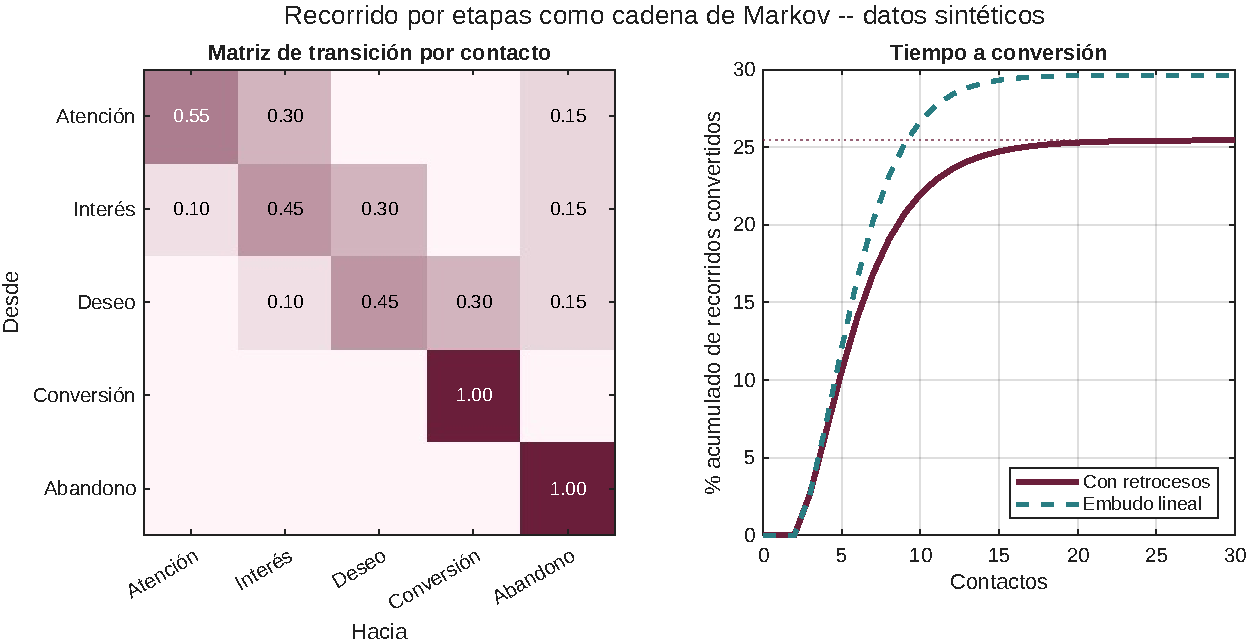
\includegraphics[width=0.95\textwidth]{figuras/matlab/cap07_markov_etapas.pdf}
  \captionof{figure}{Matriz de transición por contacto y tiempo a conversión
  con retrocesos y como embudo lineal. Fuente: elaboración propia con datos
  sintéticos.}
  \label{fig:cap07-markov}
\end{center}

\begin{center}
  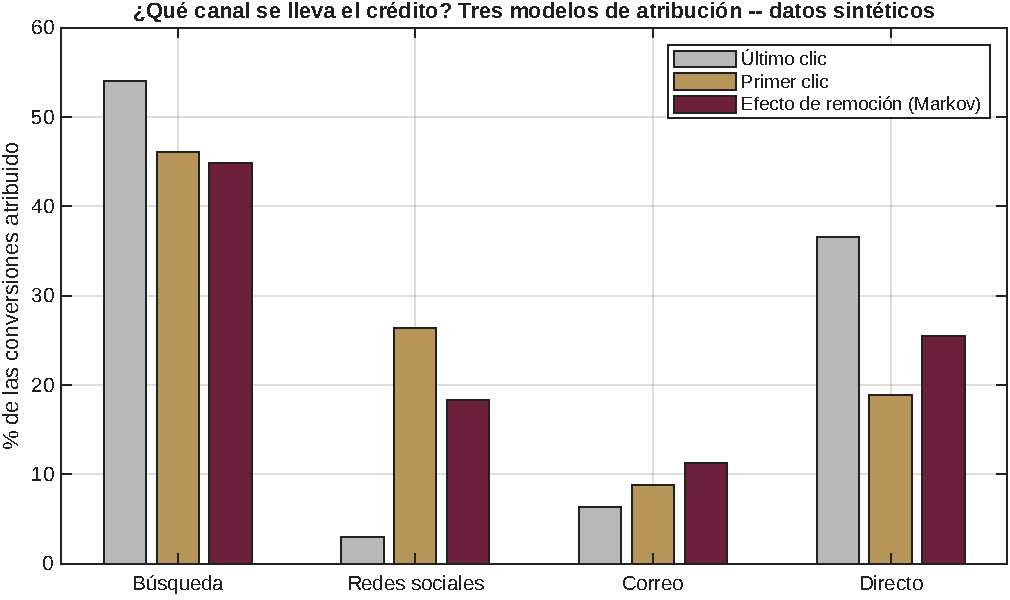
\includegraphics[width=0.85\textwidth]{figuras/matlab/cap07_atribucion.pdf}
  \captionof{figure}{Crédito que recibe cada canal según tres modelos de
  atribución. Fuente: elaboración propia con datos sintéticos.}
  \label{fig:cap07-atribucion}
\end{center}

\textbf{Interpretación de negocio.} Con los valores por defecto, 25.4\,\% de
los recorridos convierte, contra 29.6\,\% del mismo recorrido sin retrocesos.
Volver atrás no solo baja la conversión: alarga el recorrido
(6.95 contactos hasta convertir, entre quienes convierten, contra 6.67) y
desplaza las conversiones hacia más tarde. Un embudo lineal que ignora esos
retrocesos sobreestima cuántos convierten y subestima cuánto tardan.

La figura~\ref{fig:cap07-atribucion} muestra algo más incómodo. Redes sociales
recibe 3.0\,\% del crédito con el último clic y 18.3\,\% con el efecto de
remoción. No cierra ventas: abre recorridos y los pasa a búsqueda. Una
organización que decide su presupuesto con el último clic recortaría el canal
que alimenta a los demás. Esta es la versión cuantitativa de la advertencia
de la sección~\ref{sec:cap07-aidas}: la acción es la etapa que mejor se mide y
por eso la que más se sobrevalora.

\textbf{Ejercicio propuesto (usen exactamente este script, solo cambien el
bloque de parámetros).} Corran el script tres veces y completen un cuadro con
la probabilidad de convertir, los contactos esperados hasta convertir (entre
quienes convierten) y el crédito de Redes sociales con el último clic y con el
efecto de remoción:
\begin{enumerate}
  \item \textbf{Caso A — valores por defecto:} los seis parámetros tal como
  están en el script.
  \item \textbf{Caso B — recorrido desordenado:} cambien \texttt{pRetroceder}
  de 0.10 a 0.25, sin tocar nada más.
  \item \textbf{Caso C — más inicio en redes y mejor tráfico directo:}
  regresen \texttt{pRetroceder} a 0.10 y cambien \texttt{inicioRedes} a 0.70 y
  \texttt{convDirecto} a 0.60.
\end{enumerate}
Con el cuadro completo, respondan por escrito: en el Caso B, ¿qué ocurre con
la conversión y con el tiempo hasta convertir, y qué le dice eso a una marca
que mide su embudo como si fuera lineal? En el Caso C, ¿cambia el crédito de
Redes sociales con el último clic? ¿Y con el efecto de remoción? Expliquen
por qué un modelo de atribución puede ser engañoso aunque sus cálculos sean
correctos.

\textbf{Extensión opcional.} Agreguen una fila y una columna a \texttt{QC}
para un quinto canal (por ejemplo, \enquote{Marketplace}) y verifiquen que el
efecto de remoción sigue sumando 100\,\% tras normalizar.

\textbf{Sin MATLAB.}
\texttt{matlab/cap07/cap07\_journey\_markov\_interactivo.html} tiene los mismos
parámetros, los casos A, B y C y el cuadro de comparación.

\textbf{Con datos propios (extensión opcional).}
\texttt{cap07\_journey\_datos\_propios.html}
estima la cadena de Markov a partir de recorridos propios (hoja «Recorridos»: una fila por recorrido, con la ruta de canales y si terminó en compra, o la ruta agrupada con una columna «Cantidad») y reparte las compras con cuatro modelos de atribución: último clic, primer clic, lineal y efecto de remoción. Los datos no salen del navegador.
\end{cajaLaboratorio}

\begin{cajaEtica}
Reconstruir el recorrido de una persona exige unir sus rastros: lo que vio en
una red social, lo que buscó, lo que abrió en el correo y lo que compró. Cada
unión reduce su anonimato. Un modelo de atribución como el del laboratorio
trabaja con recorridos \emph{agregados} y no necesita saber quién es cada
persona; un mapa individual sí. Antes de cruzar fuentes, hay que preguntar si
la finalidad lo justifica, si existe base legal para cada fuente (Cap.~3) y si
bastaría con datos agregados. Declarar los límites del mapa también es una
obligación ética: presentar como \enquote{recorrido completo} lo que es una
muestra estilizada induce a decidir con una certeza que no existe.
\end{cajaEtica}

\section{Estudio de caso}
\label{sec:cap07-caso}

\begin{casoFicticio}
Una marca mexicana de ropa deportiva vende en línea. Su informe de atribución
usa \enquote{último clic} y concluye que redes sociales aporta 3\,\% de las
ventas, búsqueda 54\,\% y tráfico directo 37\,\%. La dirección decide pasar el
presupuesto de redes sociales a búsqueda de pago. Tres meses después, las
ventas totales bajan y el costo por clic de búsqueda sube.

Un analista reconstruye los recorridos con una cadena de Markov y calcula el
efecto de remoción: si se apagara redes sociales, la probabilidad global de
convertir caería cerca de una quinta parte. Nadie había medido eso.

\textbf{Preguntas guía.}
\begin{enumerate}
  \item ¿Por qué el último clic casi no acredita a redes sociales? ¿Qué papel
  juega el canal en el recorrido?
  \item Explique con el lenguaje del capítulo por qué las ventas bajaron y el
  costo de búsqueda subió.
  \item Señale una limitación del efecto de remoción como medida de
  \enquote{causa}. ¿Qué experimento diseñaría para confirmarlo?
  \item ¿Qué datos de identidad necesitaría cruzar el analista y qué
  obligaciones legales implican (Cap.~3)?
\end{enumerate}
\end{casoFicticio}

\section{Actividades y evidencias del portafolio}

Estas actividades hacen crecer el entregable único de la práctica
\enquote{Recorrido del consumidor digital}, que inició en el Cap.~6.

\begin{description}
  \item[Infografía colaborativa] Representar el \textit{customer journey} del
  caso real elegido en el Cap.~6, con las cinco etapas AIDAS, los puntos de
  contacto y las métricas de cada una (cuadro~\ref{tab:cap07-aidas}).
  \item[Participación en wiki de mapeo del \textit{customer journey}] Subir a
  la wiki del grupo el mapa de recorrido del caso (figura~\ref{fig:cap07-mapa}
  como punto de partida), con emoción, dato que deja y oportunidad por etapa,
  y comentar el mapa de otro equipo.
  \item[Solución de casos] Resolver por escrito el estudio de caso de la marca
  de ropa deportiva (sección~\ref{sec:cap07-caso}).
  \item[Reporte de práctica] Incluir el cuadro de los tres casos del
  laboratorio y las respuestas de comparación en el entregable único de la
  práctica.
\end{description}

\section{Ruta de aprendizaje autónomo}

Dos horas de aprendizaje autónomo. Tareas concretas:
\begin{enumerate}
  \item Ejecutar \texttt{cap07\_journey\_markov\_interactivo.html}, completar
  el cuadro de los casos A, B y C y anotar qué parámetro más cambia el crédito
  de Redes sociales.
  \item Marcar sobre el mapa del caso del equipo cada punto de contacto como
  de la marca, de socios, del cliente o social/externo, siguiendo a
  \textcite{lemon2016}.
  \item Elegir uno de los marcos del cuadro~\ref{tab:cap07-marcos} y redactar
  media cuartilla sobre quién lo produjo y qué intereses tenía.
  \item (Opcional) Con \texttt{cap07\_journey\_datos\_propios.html} (opcional), cargar el \textbf{Ejemplo 2} (tienda de ropa) y escribir en dos líneas qué canal se subestima con el último clic.
\end{enumerate}

\section{Síntesis}

El recorrido del consumidor se organiza en cinco etapas (atención, interés,
deseo, acción y satisfacción) que la mercadotecnia digital traduce a puntos
de contacto, datos y métricas. El modelo que las ordena, AIDA, tiene una
genealogía más débil de lo que se cree, y los marcos que lo sustituyen
(recorrido de decisión, \textit{messy middle}, 5A) son aportes de consultoras
y plataformas con valor pedagógico y sin validación independiente, aunque la
crítica al embudo lineal sí tiene respaldo académico. Un mapa de recorrido es
una herramienta útil y estilizada: no registra el camino real de una persona.
Modelar el recorrido como cadena de Markov permite cuantificar el costo de los
retrocesos y repartir el crédito de las conversiones de un modo más justo que
el último clic.

\subsection*{Glosario del capítulo}
\begin{description}
  \item[AIDAS] Atención, interés, deseo, acción y satisfacción: modelo de cinco etapas del recorrido.
  \item[Cadena de Markov] Proceso en que el siguiente estado depende solo del actual.
  \item[Efecto de remoción] Caída porcentual de la probabilidad de convertir al eliminar un canal.
  \item[Estado absorbente] Estado del que no se sale (Conversión o Abandono).
  \item[Inicio en redes] Parámetro editable \texttt{inicioRedes}: fracción de recorridos que empiezan en redes sociales. Rango: real entre 0 y 1; los casos didácticos usan 0.40 y 0.70.
  \item[\textit{Messy middle}] Tramo entre el disparador y la compra, descrito como ir y venir entre explorar y evaluar.
  \item[Probabilidad de abandonar] Parámetro editable \texttt{pAbandonar}: probabilidad por contacto de salir del recorrido. Rango: real entre 0 y 1, con \texttt{pAvanzar} $+$ \texttt{pRetroceder} $+$ \texttt{pAbandonar} $\le 1$; el libro usa 0.15.
  \item[Probabilidad de avanzar] Parámetro editable \texttt{pAvanzar}: probabilidad por contacto de pasar a la siguiente etapa. Rango: real mayor que 0 y hasta 1; el libro usa 0.30.
  \item[Probabilidad de retroceder] Parámetro editable \texttt{pRetroceder}: probabilidad por contacto de volver a la etapa anterior. Rango: real entre 0 y 1 (0 equivale a un embudo lineal); los casos didácticos usan 0.10 y 0.25.
  \item[Último clic / primer clic] Reglas de atribución que dan todo el crédito al último o al primer canal del recorrido.
\end{description}

\subsection*{Autoevaluación}

\textbf{Opción múltiple}

\begin{enumerate}
  \item Según la investigación histórica más reciente citada en el capítulo,
  la atribución de AIDA a Lewis (1898):
  \begin{enumerate}
    \item[a)] Está plenamente documentada con fuentes primarias.
    \item[b)] Se apoya en una fuente secundaria de 1925 y carece de evidencia primaria. \textit{(correcta)}
    \item[c)] Fue formulada en 1921 por Sheldon.
    \item[d)] No ha sido discutida nunca.
  \end{enumerate}
  \textit{Justificación:} caso de apertura.

  \item La crítica al embudo lineal como descripción de la conducta real:
  \begin{enumerate}
    \item[a)] Solo la sostiene Google con su estudio propietario.
    \item[b)] Tiene respaldo académico independiente, aunque los modelos de marca sean investigación de consultoras o plataformas. \textit{(correcta)}
    \item[c)] No tiene ningún respaldo empírico.
    \item[d)] Se prueba con un solo experimento controlado.
  \end{enumerate}
  \textit{Justificación:} recuadro de Frontera.

  \item En el laboratorio, ¿qué mide el \enquote{efecto de remoción} de un
  canal?
  \begin{enumerate}
    \item[a)] La proporción de recorridos que terminan en ese canal.
    \item[b)] La caída de la probabilidad de convertir si se elimina ese canal. \textit{(correcta)}
    \item[c)] El costo por clic del canal.
    \item[d)] El número de contactos del canal.
  \end{enumerate}
  \textit{Justificación:} concepto detrás del código.
\end{enumerate}

\textbf{Preguntas abiertas}

\begin{enumerate}
  \item Explique por qué un mapa de recorrido \enquote{a 360 grados} de cada
  cliente es una promesa comercial y no un resultado verificado.
  \textit{Clave:} fragmentación de dispositivos e identidades, bloqueo de
  \textit{cookies}, mediación de asistentes de IA y ausencia de evidencia
  académica de que sea alcanzable (sección~\ref{sec:cap07-mapeo}).
  \item A partir de la figura~\ref{fig:cap07-atribucion}, explique por qué
  decidir el presupuesto con el último clic puede dañar las ventas.
  \textit{Clave:} los canales que abren o ayudan casi no reciben crédito y
  su recorte rompe el recorrido que alimenta a los que cierran.
\end{enumerate}

\section{Lecturas recomendadas}

\begin{description}
  \item[\textcite{iwamoto2024origenaida}] Lectura de una tarde que desmonta, con documentos, una atribución repetida durante un siglo. Modelo de rigor histórico.
  \item[\textcite{santos2021consumer}] Revisión sistemática que sitúa el recorrido de decisión en su linaje teórico. Útil para separar el marco de consultoría del respaldo académico.
  \item[\textcite{lemon2016}] Tipología de puntos de contacto y marco de experiencia a lo largo del recorrido. Base para construir un mapa propio.
  \item[\textcite{anderl2016}] Atribución con cadenas de Markov frente a las reglas de último clic, con datos reales de cuatro bases.
\end{description}
